\let\negmedspace\undefined
\let\negthickspace\undefined
\documentclass[journal]{IEEEtran}
\usepackage[a5paper, margin=10mm, onecolumn]{geometry}

\usepackage{tfrupee} 

\setlength{\headheight}{1cm} 
\setlength{\headsep }{0mm}     

\usepackage{gvv-book}
\usepackage{gvv}
\usepackage{cite}
\usepackage{amsmath,amssymb,amsfonts,amsthm}
\usepackage{algorithmic}
\usepackage{graphicx}
\usepackage{textcomp}
\usepackage{xcolor}
\usepackage{txfonts}
\usepackage{listings}
\usepackage{enumitem}
\usepackage{mathtools}
\usepackage{gensymb}
\usepackage{comment}
\usepackage[breaklinks=true]{hyperref}
\usepackage{tkz-euclide} 
\usepackage{listings}
% \usepackage{gvv}                                        
\def\inputGnumericTable{}                                 
\usepackage[latin1]{inputenc}                                
\usepackage{color}                                            
\usepackage{array}                                            
\usepackage{longtable}                                       
\usepackage{calc}                                             
\usepackage{multirow}                                         
\usepackage{hhline}                                           
\usepackage{ifthen}                                           
\usepackage{lscape}
\begin{document}

\bibliographystyle{IEEEtran}
\vspace{3cm}

\title{4.7.25}
\author{EE25BTECH11033 - Kavin}
% \maketitle
% \newpage
% \bigskip
{\let\newpage\relax\maketitle}

\renewcommand{\thefigure}{\theenumi}
\renewcommand{\thetable}{\theenumi}
\setlength{\intextsep}{10pt} % Space between text and floats
\textbf{Question}:\\
Find the points on the line $x+y=4$ which lie at a unit distance from the line $4x+3y=10$.\\
\bigskip


\textbf{Solution}:\\
According to the question,\\
\begin{align}
    \text{Equation of line $L_1$:}\ \myvec{1&1}\myvec{x\\y}=4
\end{align}
\begin{center}
    $\implies n_1^{\top} \vec{x} = c_1$
\end{center}
and
\begin{align}
    \text{Equation of line $L_2$:}\ \myvec{4&3}\myvec{x\\y}=10
\end{align}
\begin{center}
    $\implies n_2^{\top} \vec{x} = c_2$
\end{center}
The distance $\lambda$ of a vector $\vec{P}$ from the line $\vec{n_2}^{\top}\vec{x}=c_2$ is given by ,
\begin{align}
    \lambda = \frac{\abs{\vec{n_2}^{\top}\vec{P} - c_2}}{\norm{\vec{n_2}}}  
\end{align}
\begin{align}
    \lambda\norm{\vec{n_2}} = \abs{\vec{n_2}^{\top}\vec{P} - c_2} 
\end{align}
\begin{align}
    \implies\vec{n_2}^{\top}\vec{P} = c_2 \pm \lambda\norm{n_2}
\end{align}
Also, as $\vec{P}$ lies on line $L_1$,
\begin{align}
    \vec{n_1}^{\top}\vec{P} = c_1
\end{align}
On putting eqns $\brak{5}$ and $\brak{6}$ in matrix form we will get,
\begin{align}
    \myvec{n_1 & n_2}^\top\vec{P}=\myvec{c_1\\c_2\pm\lambda\norm{\vec{n_2}}}
\end{align}
where,
\begin{align*}
    \lambda = 1
\end{align*}
On substituting the values we will get,
\begin{align}
    \myvec{1&1\\4&3}\vec{P}=\myvec{4\\10\pm5}
\end{align}
with the augmented matrix followed by row reduction 
\begin{align}
	\xleftrightarrow{R_2 = R_2 - 4 R_1}\myvec{1&1 &\vrule &  4&\\ 0&-1 & \vrule& -6\pm5&}   
	\xleftrightarrow{R_2 = -R_2}\myvec{1&1&\vrule& 4& \\ 0&1 & \vrule &6\mp5} \nonumber \\
	\xleftrightarrow{R_1 = R_1-R_2}\myvec{1&0 & \vrule &-2\pm5&\\ 0&1& \vrule &6\mp5}\nonumber
\end{align}
Therefore the points on $L_1$ which lie at a unit distance from the line $L_2$ are ,
\begin{align*}
    \vec{P}=\myvec{3\\1} \ \text{and} \ \vec{P}=\myvec{-7\\11}
\end{align*}
\begin{figure}[H]
\begin{center}
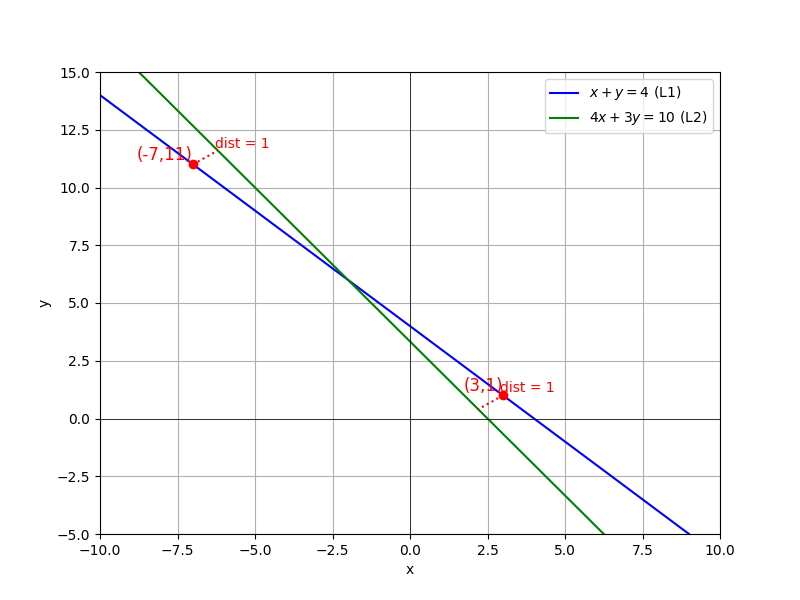
\includegraphics[width=0.6\columnwidth]{figs/fig.png}
\end{center}
\label{fig:Fig1}
\end{figure}

\end{document}


